%%%%%%%%%%%%%%%%%%%%%%%%%%%%%%%%%%%%%%%%%
% FRI Data Science_report LaTeX Template
% Version 1.0 (28/1/2020)
% 
% Jure Demšar (jure.demsar@fri.uni-lj.si)
%
% Based on MicromouseSymp article template by:
% Mathias Legrand (legrand.mathias@gmail.com) 
% With extensive modifications by:
% Antonio Valente (antonio.luis.valente@gmail.com)
%
% License:
% CC BY-NC-SA 3.0 (http://creativecommons.org/licenses/by-nc-sa/3.0/)
%
%%%%%%%%%%%%%%%%%%%%%%%%%%%%%%%%%%%%%%%%%


%----------------------------------------------------------------------------------------
%	PACKAGES AND OTHER DOCUMENT CONFIGURATIONS
%----------------------------------------------------------------------------------------
\documentclass[fleqn,moreauthors,10pt]{ds_report}
\usepackage[english]{babel}
\usepackage[most]{tcolorbox}
\usepackage{titlesec}
\usepackage{hyperref}
\makeatletter
\newcommand\setcurrentname[1]{\def\@currentlabelname{#1}}
\makeatother
\graphicspath{{fig/}}




%----------------------------------------------------------------------------------------
%	ARTICLE INFORMATION
%----------------------------------------------------------------------------------------

% Header
\JournalInfo{FRI Natural language processing course 2021}

% Interim or final report
\Archive{Project report} 
%\Archive{Final report} 

% Article title
\PaperTitle{Cross-Lingual Question Generation} 

% Authors (student competitors) and their info
\Authors{Igor Nikolaj Sok, Tian Grumerec, and Jurij Dolenc}

% Advisors
\affiliation{\textit{Advisors: Slavko Žitnik}}

% Keywords
\Keywords{Natural Language Processing, Information Retrieval, Cross-Lingual Question Generation, Doc2Query, T5 Model, Slovenian Language, SQuAD Dataset, Fine-Tuning, Multilingual NLP, Computational Linguistics}
\newcommand{\keywordname}{Keywords}


%----------------------------------------------------------------------------------------
%	ABSTRACT
%----------------------------------------------------------------------------------------

\Abstract{
This project aims to develop a Slovenian question generation model. We fine-tuned the pre-trained Doc2Query T5 model using a Slovenian translation of the SQuAD dataset and evaluated its performance in generating Slovenian questions. Additionally, we compared the results with a smaller T5 model pre-trained on Slovenian data. Our findings indicate that the fine-tuned models can produce grammatically correct and contextually relevant questions in Slovenian, though the quality of the dataset and computational constraints posed significant challenges. This report discusses the methodologies, experiments, and limitations encountered, and provides insights for future improvements in cross-lingual question generation.
}

%----------------------------------------------------------------------------------------

\begin{document}

% Makes all text pages the same height
\flushbottom 

% Print the title and abstract box
\maketitle 

% Removes page numbering from the first page
\thispagestyle{empty} 

%----------------------------------------------------------------------------------------
%	ARTICLE CONTENTS
%----------------------------------------------------------------------------------------

\section*{Introduction}
Natural language processing is currently a very actual and rapidly developing field of computer science. In the sub field of Information Retrieval (IR), there is much ongoing research that aims to improve a language models ability to understand the text and pick up its core meaning. In the scope of our project we aim to develop a model, capable of processing text and understanding it to a point, where it can provide questions based on the text in many languages. To achieve this we plan to expand on the existing Doc2Query approach and include a T5 translation model to enable cross-lingual question generation. We will manually check answers for relevance and compare the results with the answers obtained via a smaller t5 model pretrained on Slovenian language.

\subsection*{Related work}

In the article \textit{Exploring the Limits of Transfer Learning with a Unified Text-to-Text Transformer}\cite{DBLP:journals/corr/abs-1910-10683} the authors discuss a model for streamlining the task of transfer learning. Transfer learning is a procedure that enhances Natural Language Processing (NLP) by pre-training models on data-rich tasks and fine-tuning them on specific downstream tasks. The authors propose a unified framework for converting all text-based language problems into a text-to-text format. In the scope of their study they compared pre-training, unlabelled datasets, different architectures and more on many language understanding tasks and achieved state of the art results on many benchmarks including question answering and summarization. The model that achieved the best results was a T5 encoder-decoder model. They introduced a "Colosal Clean Crawled Corpus" (C4) dataset, which provides enough diverse data for general language understanding, which significantly boosts the models performance.

In the article \textit{Document Expansion by Query Prediction}\cite{DBLP:journals/corr/abs-1904-08375} the authors introduce a model called Doc2Query; a model that for a given document, predicts a query, which can then be appended to the document. The authors trained a sequence-to-sequence model that generates possible questions that the document might answer. This can be used to better index documents, to provide more accurate document search for search engines, help with Domain specific training data generation and can be used for generating pairs for a given collection of unlabelled texts. Doc2Query uses a simple seq-to-seq transformer to produce a query from the document, both of which are segmented using BPE\cite{sennrich2016neural} after being tokenized with the MOSES tokenizer. The document and queries are then truncated to avoid excessive memory usage. Once the model is trained, it predicts 10 queries using the top-k random sampling. The model was trained on the MSMARCO\cite{DBLP:journals/corr/NguyenRSGTMD16} dataset.

The article \textit{Doc2Query--: When Less is More}\cite{gospodinov2023doc2query} expands on the Doc2Query approach by trying to eliminate the "hallucinations" that Doc2Query might produce by generating questions that are not present in the source text. The authors argue that Doc2Query is prone to hallucination and that this harms retrieval effectiveness and inflates the index size. They explore and propose techniques for filtering out these harmful queries prior to indexing. Doc2Query-- estimates the relevance of a query with relevance models. With this the retrieval effectiveness of indexes improves by up to 16\%, while also reducing index size. The major drawback of this approach is the higher computational cost that arises by removing irrelevant queries.


In the article \textit{SQuAD: 100,000+ Questions for Machine Comprehension of Text}\cite{DBLP:journals/corr/RajpurkarZLL16} the authors introduce a large scale benchmark designed for evaluating machine comprehension systems. It comprises over 100000 question-answer pairs, sourced from over 500 Wikipedia articles, covering a wide range of topics. The dataset is structured such that each question is posed with reference to a specific paragraph from the corresponding article, and the answer to the question lies within that paragraph. It allows fine-grained evaluation of a models ability to understand and extract information from text.



%------------------------------------------------

\section*{Methods} 
\setcurrentname{Methods}
\label{methods} %tega mi ne brisat ker referencam section v results, ne dela

As a baseline we took the pretrained doc2query t5 model, trained on a multilingual msMarco dataset\cite{msmarcomodel}. The model is trained on 14 languages, including Russian, English, French, Italian and German. We tested the pretrained model out of the box with Slovenian queries. The results were not good. The models outputs were a mixture of different alphabets and languages, though it did pick up some structural properties of the Slovene language, probably because it also support Russian, which is a Slavic language. 

\subsection*{Fine-tuning}
For fine-tuning we utilised a Slovenian translation of the SQuAD dataset\cite{slosquad}. It is important to point out, that said dataset does not necessarily contain data, which is perfectly translated and ready for use. In fact, several question and answer pairs in the dataset semantically and grammatically do not make sense (per example "V katerem desetletju je Beyonce postal slaven?"; Beyonce is a female, referred to as a male in said passage, the decade of when she became famous does not make sense in this context). Some answers too do not make sense, but they were ignored as we focuses on question generation. But despite these flaws, the dataset was large and diverse enough to provide a good enough reference for the model to learn question generation in Slovenian.

We fine-tuned the model using the huggingface transformers library. Since the original model is available at huggingface, this made the whole fine-tuning process more streamlined and convenient. To ease the process further, we uploaded the Slovenian squad translation to huggingface, in order to access it easily, using their python datasets package. 

The first part of the training process was the preprocessing of the data. Since the Slovenian SQuAD translation dataset includes other fields, such as answers, titles and answer positions, we had to prune the dataset to only include context and question pairs. Data of such format is suitable for seq2seq fine-tuning. After that we fed the data into the Seq2Seq trainer class along with our pretrained model. We set the trainers learning rate to $2*10^-5$, per device batch size to 4 and weight decay to 0.01. We trained the model for a total of 3 epochs.

\subsection*{Further experiments}
After obtaining results from the pretrained doc2query t5 model, we wanted to compare them to results we would get if we took a model, pretrained on Slovene as a baseline. We utilised a small t5 model, trained on Slovene data\cite{slot5}. The model has about 60 million parameters, and was trained on a range of Slovenian text data. This model was much smaller than the doc2query t5 model, which uses mt5\cite{DBLP:journals/corr/abs-2010-11934} as a base, which has 300M-13B parameters. We hoped, that a model pretrained on Slovenian would be capable of understanding grammatical structure and Slovenian context better than a model pretrained on other languages. The same training parameters as for the previous model were used in the fine-tuning.


\subsection*{Limitations}
During training and evaluation we encountered many difficulties, most of them relating to the Slovenian SQuAD translation. At the start we already noticed, that the dataset is not grammatically perfect, but this issue was exemplified further during training and testing. Many translations do not make sense, or the provided answers make little sense, which showed greatly during evaluation. Questions that were generated from a badly translated text were hard to evaluate, since the initial paragraph made little sense. Examples of such passages will be presented in the results\nameref{results} section.



\section*{Results}
\setcurrentname{Results}
\label{results}

The initial results of the fine-tuned model are promising. When context from the validation set is inserted into the model, it produces questions in Slovene, whereas before fine-tuning they were a mixture of languages and alphabets, mainly Russian. The questions do cover the topic in the context, but they tend to focus on some very specific aspects of the context or give questions that are grammatically a bit lacking. This might be the result of the Slovenian SQuAD translation having similar grammatical errors. When the model is fed passages from the Slovenian Wikipedia, it provides questions that make sense and are true to the topic.

We proceeded by taking random 100 paragraphs from used database \cite{slosquad}. All 10 generated questions was manually evaluated for all 100 paragraphs by three different people. As mentioned above, initial results, when not checked properly showed promise, but actual results were not as good as we first thought. 

\subsection*{Doc2query results}
Doc2query results before fine-tuning as already mentioned were mixture of different languages like Russian. When we fine-tuned it for Slovenian language the generated questions were better. No foreign words were detected. However, the model still had issues with understanding the context. The questions often did not have any sense either because it combined wrong parts of context together or used completely wrong words. Some examples of such questions:

\begin{tcolorbox}[colback=lightgray,colframe=gray!75!black, title=Example 1, label=example:ex1]

\textbf{Beam Outputs:}
\begin{enumerate}
    \item Kdo je dokazal, da je zrak potreben za zgorevanje?
    \item V katerem letu je Robert Boyle dokazal, da je zrak potreben za zgorevanje?
    \item Kdo je dokazal, da je nitroaereus potreben za zgorevanje?
    \item V katerem letu je Robert Boyle dokazal, da je zrak potreben pri dihanju?
    \item V katerem letu je Robert Boyle dokazal, da je zrak potreben?
\end{enumerate}
\textbf{Sampling Outputs:}
\begin{enumerate}
    \item Kako visoko je bilo vetrovno vetrovno vetrovno zaradi ventilatorja?
    \item Kdo je ugotovil, da voda potrebuje čim višji volumen zraka?
    \item Na katerem mestu je John Mayow dostril, da se je zrak potrebil za zgorevanje?
    \item Kaj je bila zadnji korake, v katerem letu je John Mayow dokazal, da je zrak potreben?
    \item V katerem letu je John Mayow dokazal, da je ogenj potreben za zgorevanje?
\end{enumerate}
\end{tcolorbox}

Final Doc2query results can be seen in histogram \ref{fig:h1}.
\begin{figure}[htp!]
    \centering
    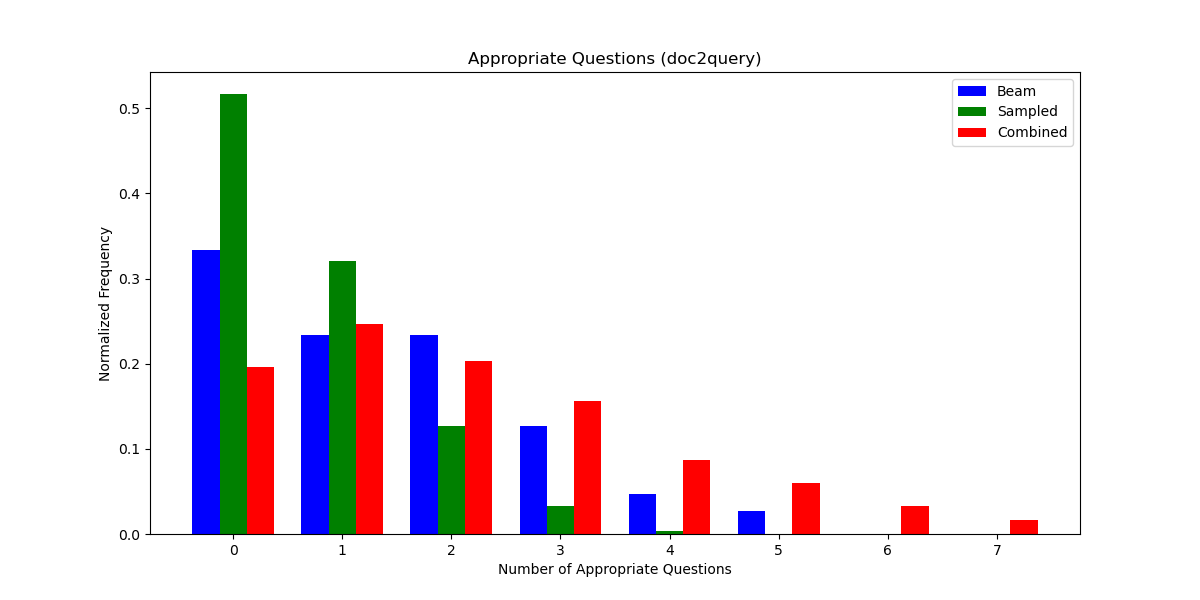
\includegraphics[width=1\columnwidth]{doc2query_combined_histogram.png}
    \caption{Doc2query results}
    \label{fig:h1}
\end{figure}
The model training took around 8 hours as it is quite large, but that is largely an issue due to the fact that we had problems training it on GPU and therefore trained it on CPU. Doc2query's average scores are listed in table \ref{tab:doc2query}.
\begin{table}[h!]
\centering
\begin{tabular}{@{}lll@{}}
\toprule
\textbf{Metric} & \textbf{Value} \\ \midrule
beam & 1.4  \\
sampled & 0.687 \\
combined & 2.08  \\ \bottomrule
\end{tabular}
\caption{Evaluation Metrics for Doc2query}
\label{tab:doc2query}
\end{table}
\subsection*{Slot5 results}
Results gotten with Slot5 model had no issues whatsoever regarding foreign words as Doc2query. It is specialised for Slovenian language and we used the small slot5 model so the training took only about 2 hours. Even though the results were visibly better than with Doc2query it still had issues with understanding context and generating questions that make sense. We must emphasise again, that the main cause for this was poor dataset . Number of positively evaluated questions (seen in table \ref{tab:slot5}) was still way below 5 on average.
\begin{table}[h!]
\centering
\begin{tabular}{@{}lll@{}}
\toprule
\textbf{Metric} & \textbf{Value} \\ \midrule
beam & 2.2  \\
sampled & 1.28 \\
combined & 3.48  \\ \bottomrule
\end{tabular}
\caption{Evaluation Metrics for Slot5}
\label{tab:slot5}
\end{table}
Final Slot5 results can be seen in histogram \ref{fig:h2}.
\begin{figure}[htp!]
    \centering
    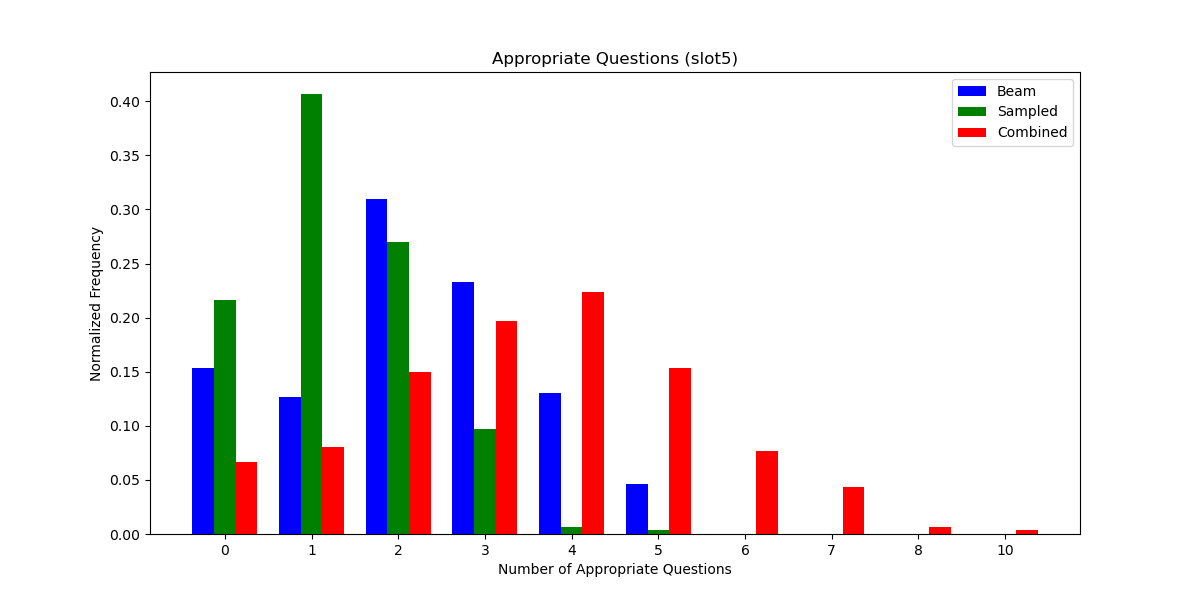
\includegraphics[width=1\columnwidth]{t5_combined_histogram.png}
    \caption{Slot5 results}
    \label{fig:h2}
\end{figure}


\subsection*{Dataset issues}
As already mentioned in section \nameref{methods} we had issues due to bad quality of the database making it hard to properly evaluate if an answer makes sense based on context or not. Here are some examples of such paragraphs that were the main cause that the questions did not make sense either:

\begin{tcolorbox}[colback=lightgray,colframe=gray!75!black, title=Example 2, label=example:ex3]
Športi na kolidžu so priljubljeni tudi v južni Kaliforniji. UCLA Bruins in USC Trojanci obe terenski ekipi v NCAA Division I v Pac-12 konferenci, in obstaja dolgoletno rivalstvo med šolami.
\end{tcolorbox}
\begin{tcolorbox}[colback=lightgray,colframe=gray!75!black, title=Example 3, label=example:ex2]
Črna smrt naj bi izvirala iz sušnih ravnic Srednje Azije, kjer je nato potovala po svileni cesti in dosegla Krim leta 1343. Od tam so ga najverjetneje nosile orientalske podgane, ki so živele na črnih podganah, ki so bile redne potnike na trgovskih ladjah. Ocenjuje se, da je črna smrt, ki se širi po vsem Sredozemlju in Evropi, ubila od 30 do 60 \% celotnega evropskega prebivalstva. Skupno je kuga zmanjšala svetovno prebivalstvo s približno 450 milijonov na 350–375 milijonov v 14. stoletju. Svetovno prebivalstvo kot celota se ni opomoglo do ravni pred kugo do 17. stoletja. Kuga se je v Evropi občasno ponavljala do 19. stoletja.
\end{tcolorbox}


\begin{tcolorbox}[colback=lightgray,colframe=gray!75!black, title=Example 4, label=example:ex4]
Seveda imajo nekateri razredi kompleksnosti zapletene opredelitve, ki ne spadajo v ta okvir. Tipičen razred kompleksnosti ima tako opredelitev, kot je naslednja:
\end{tcolorbox}
If we disregard all the bad examples of paragraphs, we noticed that the models had most issues when it came to mathematical definitions, formulas and explanations. Examples 456 show such paragraphs and corresponding answers. Example below shows some of the generated questions to a paragraph (paragraph was incorrectly translated).

\begin{tcolorbox}[colback=lightgray,colframe=gray!75!black, title=Example 5, label=example:ex5]
Beam Outputs:
\begin{itemize}
    \item Kaj se zgodi, ko je minilo večkratnik 9?
    \item Koliko praštevil je v vseh drugih vrsticah?
    \item Koliko praštevilk je v vseh drugih vrsticah?
    \item Koliko praštevil je v vseh drugih vrsticah?
    \item Kaj se zgodi, ko je minilo večkratnik 9.?
    \item Kaj je največja količina praštevilk?
    \item Kakšno je razmerje med številom vseh praštevil?
    \item Kaj se imenuje stopnja, ki je enaka nič v vseh drugih vrsticah?
    \item V kateri vrstici se začne število?
    \item Kaj je največja skupna praštevilka, ki je v vrstici 9?
\end{itemize}

\end{tcolorbox}


Slot5 was significantly better than Doc2query. Grammatical improvement was noticed immediately. That is mainly because it is trained specifically for Slovenian language on Slovenian datasets, meanwhile Doc2query is trained on different datasets from different languages.



%------------------------------------------------

\section*{Discussion}

The fine-tuned Doc2query model showed improvements in Slovenian questions compared to the pre-trained model, the SloT5 models, trained on Slovenian data, produced more grammatically correct and relevant questions, which shows why using language-specific training data is important. Performance metrics(average scores for beam and sampled outputs) show some success in the Doc2query model but we see there is still a lot of room for improvement, especially in understanding the context. SloT5 scores show that the model is much better at handling Slovenian text, but it still struggles with complex statements and poor translations.

Through our work, we faced many challenges, one of which was the dataset quality. The Slovenian SQuAD dataset had many grammatical errors and poor translations, which affected the model's training and evaluation. The generated questions were often nonsensical, impacting the reliability of the results.  We also faced issues in context understanding, both models showed difficulties in comprehending the context, which often lead to generating incorrect questions. This was especially true where paragraphs included complex concepts or mathematical definitions. One of the things holding us back were also the computational Constraints. Most of the training was done on CPUs, and not GPUs, which significantly extended the need training time. That means there was less time and options for experimentation and fine-tuning. Training on GPUs would allow us to optimize and fine-tune our models more extensively.

To improve our work, we could spend some time in cleaning/corrections the SQuAD dataset, which would likely give us better training results.  Better use of computational resources (using GPUs) would give us more time for experimentation and help us explore different model parameters more extensively. In the future, we could expand the datasets which would offer better our model's performance. In terms of evaluation techniques, we could look into automated evaluation techniques to provide us with more metrics and try to objectively assess the generated questions.

In conclusions, in this project we successfully demonstrated the possibility of fine-tuning pre-trained models for cross-lingual question generation in Slovenian. The results shown were promising but there are still various improvements and implementations that could enhance our model's performance.
%------------------------------------------------



%----------------------------------------------------------------------------------------
%	REFERENCE LIST
%----------------------------------------------------------------------------------------
\bibliographystyle{unsrt}
\bibliography{report}


\end{document}